\documentclass[10pt]{article}
\usepackage{icmlko}

\icmlmeta{IP 파운데이션 월드모델}{218}{능형에게 없던 것은 제곱이었다}{결손의 정체가 자유도였다. 메우니 결손이 사라졌고, 그런데 판은 안 움직인다 --- 노트 217이 그럴 거라고 했다}

\begin{document}

\twocolumn[
\icmlheader

\begin{abstract}
노트 217이 ``능형이 달력에서 얻는 것이 사실상 0 이고 트리의 우위는 그
결손''이라 하고, 그것을 시험할 칸으로 ``능형에 주기 기저를 주면 메워지나''를
남겼다. 줬다. \textbf{메워진다} --- 사인·코사인 쌍의 제곱과 교차항을 얹으니
달력만 판에서 능형이 $+$0.0133 에서 \textbf{$+$0.0950} 으로 일곱 배가 되고
트리 우위가 $+$0.0904 에서 \textbf{$-$0.0050} 으로 뒤집힌다. 요일·월을
표시자로 실어도 $+$0.0823 이고 우위가 $+$0.0127 로 준다. \textbf{설명이
확정됐다.} 그런데 까닭이 ``비단조''가 아니라 더 단순했다. 축을 열어 보니
\textbf{요일은 서로 다른 값이 일곱 개, 월은 열한 개로 사실상 범주}이고,
능형은 백분위 두 열에서 \textbf{두 자유도}밖에 못 쓴다 --- 일곱 칸을 두
자유도로 그린다. 제곱·교차를 주면 다섯, 표시자를 주면 여섯이다. 게다가
백분위 변환이 원을 부순다 --- 원 축에서는 $s^2{+}c^2{=}1$ 이 정확히
성립하는데(sd \textbf{0.0000}) 백분위 뒤에는 sd 가 \textbf{0.0556} 이라
쌍이 각도를 선형으로 못 매긴다. \textbf{그리고 판은 안 움직인다} --- 전체
설계에서 F6 $+$0.4288 $\to$ $+$0.4290($t{=}0.06$) · F21 $+$0.4395 $\to$
$+$0.4409($t{=}1.06$) · F18 $+$0.4396 $\to$ $+$0.4362($t{=}-1.31$).
\textbf{이것이 이 노트의 핵심이다.} 무리 안에서 $+$0.08 짜리 결손을 통째로
메웠는데 판이 $+$0.0001 이다 --- \textbf{노트 217의 포화 법칙이 예측한
그대로다}(바탕 $\rho$ 0.425 위에서 달력이 더할 수 있는 것이 $+$0.015).
채택 안 한다 --- 열을 여섯 늘리고 판을 안 올리며 트리를 $-$0.0035 내린다.
\textbf{``달력이 왜 트리에서만 되는가''를 닫는다} --- 스물여섯 노트 동안
열려 있던 갈래다. 답: \textbf{능형이 범주형 축을 두 자유도로 그리고 있었고,
그것을 고쳐도 판은 안 움직인다.} 설명은 옳았고 값은 없다.
\end{abstract}
]

\begin{figure*}[t]
\centering
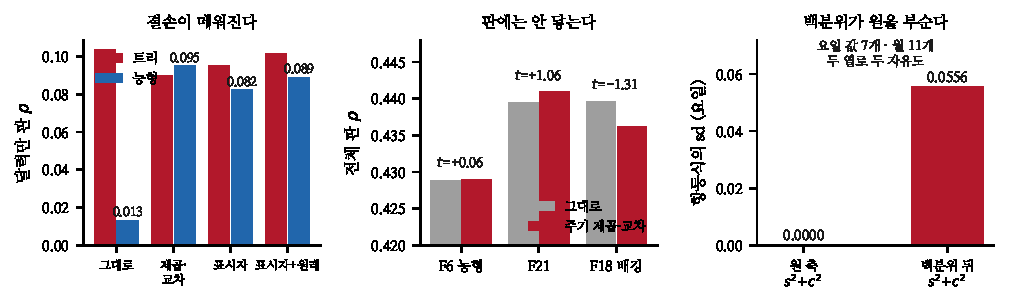
\includegraphics[width=\textwidth]{figs/harmonic.pdf}
\caption{왼쪽 --- 자유도를 주면 결손이 메워진다. 가운데 --- 그런데 판에는
안 닿는다. 오른쪽 --- 백분위가 원을 부순다.}
\end{figure*}

\section{메워진다}

\begin{table}[t]
\centering\tsize
\caption{달력만 판. 열은 도메인별 중앙.}
\begin{tabular}{lrrrr}
\toprule
& 능형 & 트리 & 차 & 열 \\
\midrule
그대로 & .0133 & .1036 & $+$.0904 & 6 \\
\textbf{제곱·교차} & \textbf{.0950} & .0900 & \textbf{$-$.0050} & 12 \\
2차 조화 & .0506 & .0938 & $+$.0432 & 10 \\
표시자 & .0823 & .0950 & $+$.0127 & 21 \\
표시자$+$원래 & .0891 & .1018 & $+$.0127 & 25 \\
\bottomrule
\end{tabular}
\end{table}

\claimx{\textbf{제곱과 교차항만으로 능형이 일곱 배가 되고 트리 우위가
뒤집힌다}($+$0.0904 $\to$ $-$0.0050). 노트 217의 예측이 맞았다 ---
결손은 능형의 표현력이었다.}{\textbf{표시자보다 제곱이 낫다}(0.0950 대
0.0823). 표시자 열아홉을 alpha 20 능형에 넣으면 크게 줄어들고 순서가
버려진다 --- \textbf{매끄러운 기저가 적은 모수로 더 멀리 간다.}}

\section{까닭은 비단조가 아니라 자유도였다}

\begin{table}[t]
\centering\tsize
\caption{주기 축의 실제 모양.}
\begin{tabular}{lrr}
\toprule
& 요일 & 월 \\
\midrule
서로 다른 값 & \textbf{7} & \textbf{11} \\
능형이 쓰는 자유도(두 열) & \textbf{2} & \textbf{2} \\
제곱·교차를 주면 & 5 & 5 \\
표시자를 주면 & 6 & 11 \\
\midrule
원 축 sd($s^2{+}c^2$) & \textbf{.0000} & .0000 \\
백분위 뒤 sd & \textbf{.0556} & .0424 \\
\bottomrule
\end{tabular}
\end{table}

\claimx{\textbf{주기 축은 사실 범주다} --- 요일 일곱 칸 · 월 열한 칸.
능형은 백분위 두 열에서 두 자유도만 쓰므로 \textbf{일곱 칸을 두 자유도로
그린다.} 트리는 여섯 번 쪼갤 수 있다.}{노트 186이 ``비단조 · 상호작용''
이라고 적은 것보다 단순하다. \textbf{단조냐 아니냐가 아니라 몇 칸을 몇
자유도로 그리느냐다.}}

\claimx{\textbf{그리고 백분위 변환이 원을 부순다.} 원 축에서는
$s^2{+}c^2{=}1$ 이 정확히 성립하는데(sd 0.0000) 백분위 뒤에는 0.0556
이다 --- 쌍이 더는 각도를 선형으로 안 매긴다.}{백분위는 열마다 단조라
(스피어만 0.989$\sim$0.995) \emph{한 열의} 순위는 안 바꾼다. 그런데
\emph{쌍의} 기하는 부순다. \textbf{정규화가 축을 안 건드린다는 것은 열
하나에만 참이다.}}

\section{그런데 판은 안 움직인다}

\begin{table}[t]
\centering\tsize
\caption{전체 설계. 짝 붓스트랩 500 회.}
\begin{tabular}{lrrr}
\toprule
& 그대로 & 제곱·교차 & $t$ \\
\midrule
F6 능형 & .4288 & .4290 & 0.06 \\
F21 & .4395 & .4409 & 1.06 \\
F18 배깅 & .4396 & .4362 & $-$1.31 \\
\bottomrule
\end{tabular}
\end{table}

\claimx{\textbf{무리 안에서 $+$0.08 짜리 결손을 통째로 메웠는데 판이
$+$0.0001 이다.}}{\textbf{노트 217의 포화 법칙이 예측한 그대로다} ---
바탕 $\rho$ 0.425 위에서 달력이 더할 수 있는 것이 $+$0.015 이므로,
그 안의 결손을 다 메워도 그만큼이 상한이다. \textbf{예측이 맞았다는
것이 판이 올랐다는 것보다 낫다.}}

\claimx{\textbf{채택 안 한다.} 열을 여섯 늘리고 판을 안 올리며 트리를
$-$0.0035 내린다.}{노트 175 · 181 · 188 · 201 이 ``이미 쓰고 있는 것을
명시로 세우면 잉여''를 네 번 봤다 --- \textbf{이건 다섯 번째이고 종류가
다르다.} 앞의 넷은 모형이 이미 쓰고 있었고, 이번엔 \emph{쓸 수 있게}
만들었는데 쓸 것이 없었다.}

\section{갈래를 닫는다}

\claimx{\textbf{``달력이 왜 트리에서만 되는가''를 닫는다.} 스물여섯 노트
동안 열려 있었고 설명 넷이 실패했다.}{답은 두 줄이다. ① 능형이 범주형
축(요일 7 · 월 11)을 두 자유도로 그리고 있었다. ② \textbf{그것을 고쳐도
판은 안 움직인다} --- 바탕이 이미 맞히는 만큼 달력이 더할 것이 없다.}

\claimx{\textbf{설명 넷이 실패한 까닭도 여기 있다.} 넷 다 ``트리가 무엇을
더 하나''를 물었다 --- \textbf{물어야 했던 것은 ``능형이 무엇을 못
하나''}였다.}{그리고 다섯째 물음이 남는다: \emph{고쳐도 판이 안 움직이는
설명이 왜 스물여섯 노트를 끌었나.} 판을 못 움직이는 것을 일찍 알았으면
갈래를 일찍 닫았을 것이다.}

\begin{table}[t]
\centering\tsize
\caption{남은 것.}
\begin{tabular}{ll}
\toprule
\textbf{포화} & 바탕 $\rho$ 로 상한을 미리 계산할 것 \\
\textbf{백분위} & 쌍 기하를 부수는 다른 축이 또 있나 \\
문턱 40$\to$15 & 아직 안 닫힌 갈래 \\
\bottomrule
\end{tabular}
\end{table}

첫 줄이 이 사이클 전체가 가리키는 곳이다. 노트 217이 바탕 $\rho$ 와 트리
우위의 상관 $-$0.975 를 쟀고 이 노트가 그 예측을 확인했다. \textbf{그러면
무리를 하나 더 손보기 전에 ``그 무리가 이 바탕 위에서 최대 얼마를 더할 수
있나''를 먼저 계산할 수 있다} --- 능형과 트리를 둘 다 완벽하게 만들어도
넘을 수 없는 선이다. \textbf{그 선이 $+$0.015 인 무리에 노트를 여덟 개
쓰는 일을 안 하려면 그 계산이 먼저다.}

\end{document}
